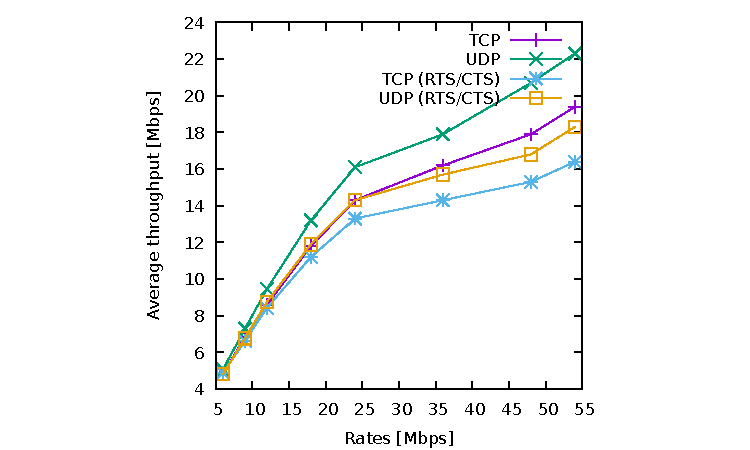
\includegraphics[width=0.5\textwidth]{traces/L3-3-1-tput.pdf}
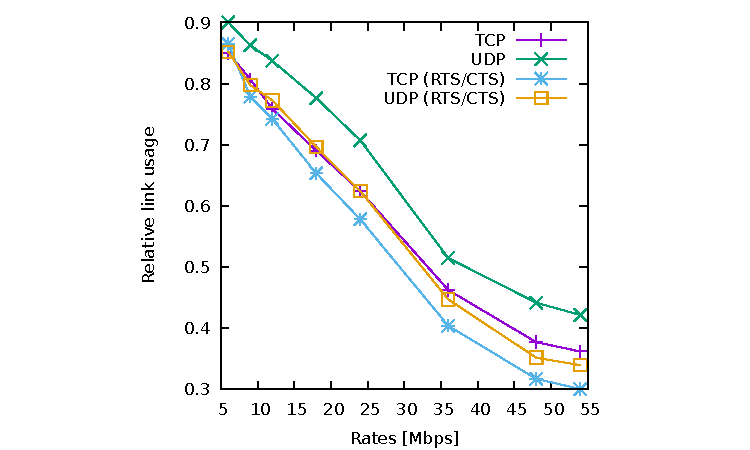
\includegraphics[width=0.5\textwidth]{traces/L3-3-1-usage.pdf}

For both TCP and UDP throughput is consistently lower with RTS/CTS enabled. The only communication in our tests is direct traffic between STA1 and AP (only STA1 $\rightarrow$ AP in case of UDP). There were few collisions even without RTS/CTS. This means RTS/CTS mainly adds overhead, leading to lower throughput. \\ \\ Even with RTS/CTS enabled UDP still outperforms TCP: TCP's lower performance is caused by its additional overhead and congestion control, which is not changed by having RTS/CTS enabled.
